\subsection{Angular power spectra in the Limber approximation}
%
% Given that we are interested in sub-degree and degree angular scales (\ell >> 10), we can safely adopt the so-called Limber approximation
%
% Our focus will be on small angular scales (high \ell), where the signal to noise is highest and the effects of quasi-linear evolution become important. This allows us to make the Limber approximation, which in our context is
%
% On small angular scales (high \ell) one may make the Limber approximation [44], under which C_{\ell} reduces to a single integral of the equal-time, real-space power spectrum:
%
% Because the relevant angular scales are much smaller than 1 radian (multipoles \ell > 100), the theoretical angular cross-correlation can be computed using the Limber approximation (Limber 1953) as
%

Galaxy overdensity $\delta_g$ and CMB lensing convergence $\kappa$ are both projections of 3D density fields, expressed as line-of-sight integrals over their respective projection kernels. The angular cross-spectrum between two such fields $X$ and $Y$ is given by
%%
\begin{align}
C_{\ell}^{XY} = \int & d\chi_1 \int d\chi_2 \ W^X(\chi_1) \ W^Y(\chi_2) \nonumber \\ & \int \frac{2}{\pi}k^2dk \ P_{XY}(k;z_1,z_2) \ j_{\ell}(k\chi_1) \ j_{\ell}(k\chi_2)
\end{align}
%%
where $W^X$ and $W^Y$ are the projection kernels, $P_{XY}$ is the real-space power cross-spectrum, and $j_{\ell}$ are spherical Bessel functions of the first kind. As we are primarily interested in angular scales $\lesssim 1^{\circ}$ ($\ell \gtrsim 100$), we can adopt the Limber approximation \citep{Limber53, Rubin54} and its first order correction \citep{LoverdeAfshordi08}, under which the $k$ integral evaluates to
%%
\begin{equation}
    P_{XY}{\Big (}k = \frac{\ell + 
\nicefrac{1}{2}}{\chi_1}; z{\Big )}\frac{1}{\chi_1^2}\delta^{D}(\chi_1 - \chi_2)
\end{equation}
%%
Hence the angular cross-spectrum may be expressed as a single integral over line-of-sight co-moving distance,
%%
\begin{align}
C_{\ell}^{XY} &= \int d\chi \ W^X(\chi) W^Y(\chi) \frac{1}{\chi^2}P_{XY}{\Big (}k = \frac{\ell + 
\nicefrac{1}{2}}{\chi}; z{\Big )} \\
&= \int dz \ \frac{H(z)}{c} W^X(z) W^Y(z) \frac{1}{\chi^2}P_{XY}{\Big (}k = \frac{\ell + 
\nicefrac{1}{2}}{\chi}; z{\Big )}
\end{align}
%%
The projection kernels for galaxy overdensity and CMB lensing convergence are, respectively,
%%
\begin{gather}
\begin{aligned}
    W^{g}(z) &= \phi(z) = \frac{c}{H(z)}\phi(\chi) = \frac{c}{H(z)} W^{g}(\chi) \\
    W^{\kappa}(z) &= \frac{3}{2c} \Omega_{m0} \frac{H_0^2}{H(z)} (1+z) \frac{\chi(\chi_{\rm *}-\chi)}{\chi_{\rm *}} = \frac{c}{H(z)} W^{\kappa}(\chi)
\end{aligned}
\end{gather}
%%
where $\chi_{\rm *} = \chi(z_{\rm *}{\approx}1100) \approx 9400$ $h^{-1}$Mpc is the distance to the surface of last scattering, and $\phi(z)$ is the normalized redshift distribution of the galaxy sample. These kernels are plotted in Figure~\ref{fig:kernels}.

\begin{figure}
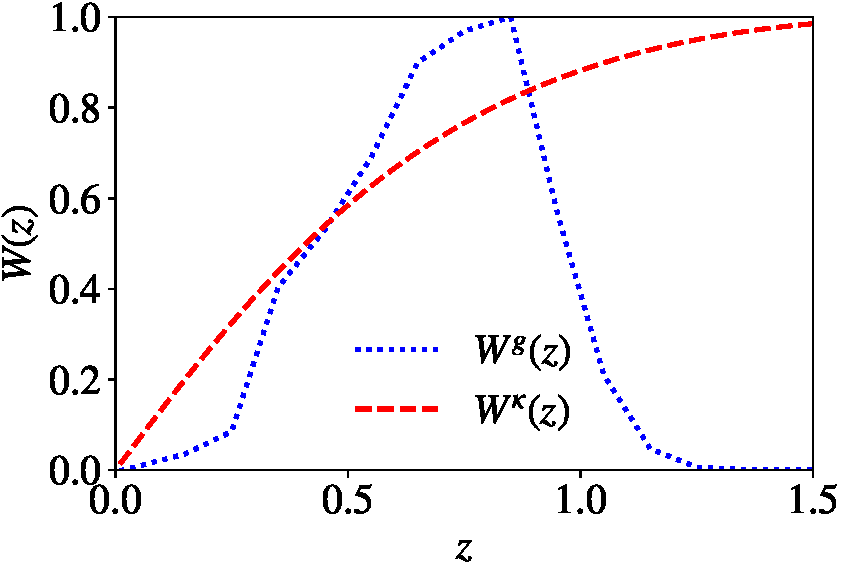
\includegraphics[width=\linewidth]{figures/windows.pdf}
\caption{Projection kernels for the galaxy sample (dashed blue line) and CMB lensing (dotted red line), both normalized to a unit maximum.}
\label{fig:kernels}
\end{figure}

Plugging in and simplifying the expressions for the spectra,
\begin{align}\label{eq:simplified_cells}
    C_{\ell}^{\rm \kappa g} &= \int d\chi \ \frac{3\Omega_{m0}H_0^2}{2c^2} \frac{1+z}{\chi^2}\frac{\chi(\chi_{\rm *}-\chi)}{\chi_{\rm *}}\phi(\chi)P_{\rm mg}{\Big (}k = \frac{\ell + 
\nicefrac{1}{2}}{\chi}; z{\Big )} \nonumber \\ %%%
    &= \int dz \ \frac{3\Omega_{m0}H_0^2}{2cH(z)} \frac{1+z}{\chi^2}\frac{\chi(\chi_{\rm *}-\chi)}{\chi_{\rm *}}\phi(z)P_{\rm mg}{\Big (}k = \frac{\ell + 
\nicefrac{1}{2}}{\chi}; z{\Big )}\nonumber \\ %%%
    C_{\ell}^{\rm gg} &= \int d\chi \ \phi(\chi)^2 \frac{1}{\chi^2} P_{\rm gg}{\Big (}k = \frac{\ell + 
\nicefrac{1}{2}}{\chi}; z{\Big )} \\ %%%
    &= \int dz \ \frac{H(z)}{c} \phi(z)^2 \frac{1}{\chi^2} P_{\rm gg}{\Big (}k = \frac{\ell + 
\nicefrac{1}{2}}{\chi}; z{\Big )} \nonumber \\ %%%
    C_{\ell}^{\kappa\kappa} &= \int d\chi \ {\Big (}\frac{3\Omega_{m0}H_0^2}{2c^2} \frac{1+z}{\chi^2}\frac{\chi(\chi_{\rm *}-\chi)}{\chi_{\rm *}}{\Big )}^2P_{\rm mm}{\Big (}k = \frac{\ell + 
\nicefrac{1}{2}}{\chi}; z{\Big )} \nonumber \\
    &= \int dz \ \frac{H(z)}{c}{\Big (}\frac{3\Omega_{m0}H_0^2}{2cH(z)} \frac{1+z}{\chi^2}\frac{\chi(\chi_{\rm *}-\chi)}{\chi_{\rm *}}{\Big )}^2P_{\rm mm}{\Big (}k = \frac{\ell + 
\nicefrac{1}{2}}{\chi}; z{\Big )} \nonumber
\end{align}

\subsection{Estimating angular power spectra}

Many different approaches for estimating angular power spectra from cosmological maps exist in the literature, including maximum likelihood estimators (\citealt{Bond++98}, \citealt{WandeltHansen03}), the optimal quadratic estimator (\citealt{Tegmark97}, \citealt{Tegmark++01}), and Bayesian sampling techniques (e.g. \citealt{Eriksen++04}, \citealt{Taylor++08}). While these methods have the advantage of recovering the unbiased power spectrum directly, they are computationally expensive to implement, particularly for the high resolution maps produced by modern experiments, since they scale as $\mathcal{O}(\ell_{\rm max}^6)$. Sub-optimal but numerically efficient pseudo-$C_{\ell}$ algorithms \citep{MASTER} are a popular alternative when dealing with multipoles $\ell > 30$ \citep{Efstathiou04a}, as they take advantage of speedy spherical harmonics transforms to recover the power spectrum in $\mathcal{O}(\ell_{\rm max}^3)$ time. Below, we briefly outline the pseudo-$C_{\ell}$ approach.

Any scalar function, $T(\hat{n})$, defined on a sphere may be expanded into spherical harmonics, $Y_{\ell m}$, with expansion coefficients $a_{\ell m}$ as
\begin{align}
    T(\hat{n}) &= \sum_{\ell=0}^{\infty} \sum_{m=-\ell}^{\ell} a_{\ell m} Y_{\ell m}(\hat{n}) \\ 
    a_{\ell m} &= \int_{4\pi}d\Omega \ T(\hat{n}) \ Y^{*}_{\ell m}(\hat{n})
\end{align}
The angular power spectrum $C_{\ell}$ measures the amplitude as a function of wavelength averaged over direction,
\begin{equation}
    C_{\ell} = \frac{1}{2\ell + 1}\sum_{m=-\ell}^{\ell} |a_{\ell m}|^2
\end{equation}
This is the observed angular power spectrum of a given Gaussian realization; the average over an ensemble of universes, $\langle C_{\ell} \rangle \equiv C_{\ell}^{\rm th}$, is specified by the physics (primordial perturbations, galaxy formation, etc.) with uncertainty due to cosmic variance given by
\begin{align}
    \sigma_{\ell}^2 = \frac{C^{\rm XX}_{\ell}C^{\rm YY}_{\ell} + (C^{\rm XY}_{\ell})^2}{2\ell + 1}
\end{align}

However, in practice, we are not dealing with measurements over the full sky, but rather a masked and weighted partial sky. We must account for the effect of the masking window function $W(\hat{n})$, which couples different $\ell$ modes and biases the estimator. Naive calculation of the spherical harmonics transform on a partial sky map produces the pseudo angular power spectrum, whose coefficients are a convolution of the mask and the true coefficients,
\begin{align}
    \tilde{C}_{\ell} &= \frac{1}{2\ell + 1}\sum_{m=-\ell}^{\ell} |\tilde{a}_{\ell m}|^2 \\
    \tilde{a}_{\ell m} &= \int_{4\pi}d\Omega \ T(\hat{n}) \ W(\hat{n}) \ Y^{*}_{\ell m}(\hat{n}) %\\
%    &= \sum_{\ell^{\prime}>0} \sum_{m^{\prime}=-\ell^{\prime}}^{\ell^{\prime}} a_{\ell^{\prime} m^{\prime}} K_{\ell m \ell^{\prime} m^{\prime}}
\end{align}
Fortunately, their ensemble averages are related simply as
\begin{equation}
    \langle \tilde{C}_{\ell} \rangle = \sum_{\ell^{\prime}=0}^{\infty} M_{\ell \ell^{\prime}} \langle C_{\ell^{\prime}} \rangle
\end{equation}
where the mode-mode coupling matrix $M$ can be determined purely from the geometry of the mask.
This $\ell$-by-$\ell$ matrix is generally singular in the case of large sky cuts. In order to perform matrix inversion, a common method is to use a set of discrete bandpower bins $L$ and assume the angular power spectrum is a step-wise function in each bin. Using this approach, the MASTER algorithm \citep{MASTER} is able to efficiently calculate and invert the $L$-by-$L$ mode-mode coupling matrix to extract the binned angular power spectrum from the binned pseudo angular power spectrum,
%
\begin{equation}
    \langle C_{L} \rangle = \sum_{L^{\prime}} M_{L L^{\prime}}^{-1} \langle \tilde{C}_{L^{\prime}} \rangle
\end{equation}
We use the implementation \texttt{NaMaster} \citep{Alonso++19} to calculate the mode-mode coupling matrix and decoupled angular power spectra in bandpower bins. Multipole resolution is limited by $\Delta \ell \approx 180^{\circ} / \phi$, where $\phi$ is the smallest dimension of the angular patch, and the minimum multipole that can be meaningfully constrained is the wavelength corresponding to this angular scale \citep{Peebles80}. Since the angular power of the mask is concentrated at large modes, dropping to below 10\% power at $\ell \sim 20$, we choose a conservative binning scheme with linearly spaced bins of size $\Delta \ell = 20$ from $\ell_{\rm min} = 30$ to $\ell_{\rm max} = 1500$. However, following the approach of \cite{Krolewski19}, we run \texttt{NaMaster} out to $\ell_{\rm max} = 6000$ to avoid power leakage near the edge of the measured range.

Evaluating the observational results requires consistent application of the same binning scheme to the theory curves. Since the theory curves are not necessarily piecewise constant, they must first be convolved with the mode-mode coupling matrix $M_{\ell\ell^{\prime}}$, then binned into the appropriate bandpowers, and then finally decoupled.

Additionally, the observed auto-spectra will be a combination of signal plus noise,
\begin{align}
    C_{L}^{\rm gg} = S_{L}^{\rm gg} + N_{L}^{\rm gg} \\
    C_{L}^{\kappa \kappa} = S_{L}^{\kappa \kappa} + N_{L}^{\kappa \kappa}
\end{align}
Here, $N^{\rm gg}$ is the shot noise of the galaxy field, approximately equal to $1/\bar{n}$ (where $\bar{n}$ is the mean number of galaxies per square steradian), while an estimate of the lensing noise $N^{\kappa \kappa}_{\ell}$ due to e.g. instrumental and atmospheric effects is provided by the Planck collaboration and binned into bandpowers using the method discussed above. In subsequent analysis, we have subtracted the noise terms from the observed auto-spectra, as well as dividing out the appropriate pixel window functions.

\subsection{Estimating covariance matrices}

The Gaussian or ``disconnected'' part of the covariance matrix, i.e. the covariance for perfectly Gaussian fields, dominates the total covariance matrix on linear and weakly nonlinear scales. While trivial to compute for full-sky fields, the exact correlations between different modes induced by a partial sky are computationally expensive to calculate, requiring $\mathcal{O}(\ell_{\rm max}^6)$ operations (\citealt{Efstathiou04b}, \citealt{Garcia++19}). A common approximation assumes that the off-diagonal elements remain negligible after mode coupling and simply modifies the diagonal elements by rescaling the number of degrees of freedom,
%\begin{align}
%    \text{Cov}(C^{\rm XY}_{\ell},C^{\rm XY}_{\ell^{\prime}})  &= (\sigma^{\rm XY}_{\ell})^2 \delta_{\ell \ell^{\prime}} \\ 
%    (\sigma^{\rm XY}_{\ell})^2 &= \frac{[C^{\rm XX}_{\ell}C^{\rm YY}_{\ell} + (C^{\rm XY}_{\ell})^2]_{\rm theory}}{2\ell + 1}\frac{1}{f_{\rm sky}}\frac{w_4}{w_2^2}
%\end{align}
\begin{align}\label{eq:cov_gen}
    \Sigma^{\rm XY}_{\ell\ell^{\prime}}  &= (\sigma^{\rm XY}_{\ell})^2 \delta_{\ell \ell^{\prime}} \\ 
    (\sigma^{\rm XY}_{\ell})^2 &= \frac{[(C^{\rm XX}_{\ell}+N^{\rm XX}_{\ell})(C^{\rm YY}_{\ell}+N^{\rm YY}_{\ell}) + (C^{\rm XY}_{\ell} + N^{\rm XY}_{\ell})^2]_{\rm th}}{f_{\rm sky}(2\ell + 1)}\frac{w_4}{w_2^2} \nonumber
\end{align}
where $f_{\rm sky}$ is the fraction of the sky masked,
\begin{equation}
    f_{\rm sky} = \int_{4\pi}d\Omega \ W(\hat{n})
\end{equation}
and $w_i$ is related to the $i$th moment as
\begin{equation}
    w_i = \frac{1}{f_{\rm sky}}\int_{4\pi}d\Omega \ W^{i}(\hat{n})
\end{equation}
The factor $f_{\rm sky}w_2^2/w_4$ accounts for the loss of modes induced by masking. This analytic expression has been shown to reproduce errors that are nearly identical to those obtained from Monte Carlo simulations \citep{MASTER}.

We average over the bandpower bins with the inverse weighting
\begin{align}
    \frac{1}{(\sigma_{L}^{\rm XY})^2} &= \frac{1}{\Delta \ell} \sum_{\ell \in L} \frac{1}{(\sigma_{\ell}^{\rm XY})^2}
\end{align}
where $\Delta \ell$ is the width of the bandpower bin.

\subsection{Pixelised maps and masks}

To create the galaxy density map, we pixelise the sky using the \texttt{HEALPix} scheme with resolution $N_{\rm SIDE} = 512$, corresponding to a pixel area of approximately $0.013$ square degrees. This resolution was chosen to avoid the shot noise limit in which most pixels contain zero or one galaxies (for our sample with mean density $\approx 610$ per square degree, it produces an average of 5-10 galaxies per pixel), while still probing the scales of interest, $\ell_{\rm max} \sim 3 \times N_{\rm SIDE} \approx 1500$. Using galaxy and random catalogs with the masks of Section~\ref{sec:data:masks} applied to both, we calculate the density contrast $\delta = n/\bar{n} - 1$ within each pixel. Under the \texttt{HEALPix} scheme, pixels have identical areas; however, the effective area of some pixels may be less than this if they straddle the irregular shape of the footprint boundary or overlap with masked regions around bright stars, large galaxies, etc. Since our masks are applied to both the galaxy and random catalogs in a consistent manner, we can use the random catalog to estimate the effective area of each pixel, and thus calculate accurate mean galaxy densities even in pixels that are partially masked.

To construct the pixelised galaxy mask, we measure where the distribution of effective areas deviates from a Poisson distribution, since the effective areas are estimated directly from the number of randoms per pixel, which is a Poisson process. We determine a cutoff of $a_{\rm eff}/a_{\rm tot} = 0.5$, and confirm that the pixels below this cutoff lie mainly along footprint boundary, as shown in Figure~\ref{fig:desi_mask}. Here, the effective area is calculated by using the random catalog \textit{pre}-masking, hence why the distribution is centered at $a_{\rm eff}/a_{\rm tot} \approx 1$. The equivalent distribution calculated using masked randoms results in a slightly lower mean $\tilde{a}_{\rm eff}/a_{\rm tot} \approx 0.95$ (matching the masked sky fraction of Table~\ref{tab:masks}) and an enhanced left tail since a substantial fraction of pixels are now partially masked. However, we do not necessarily need to discard these partially masked pixels as long as we are able to accurately estimate the density within them, since the pixelisation smooths the density on scales smaller than the pixel size. Hence, for our binary pixel mask, we use the cutoff calculated using the unmasked randoms, with the mask set to $1$ for $a_{\rm eff}/a_{\rm tot} > 0.5$ and 0 otherwise.

\begin{figure}
    \centering
    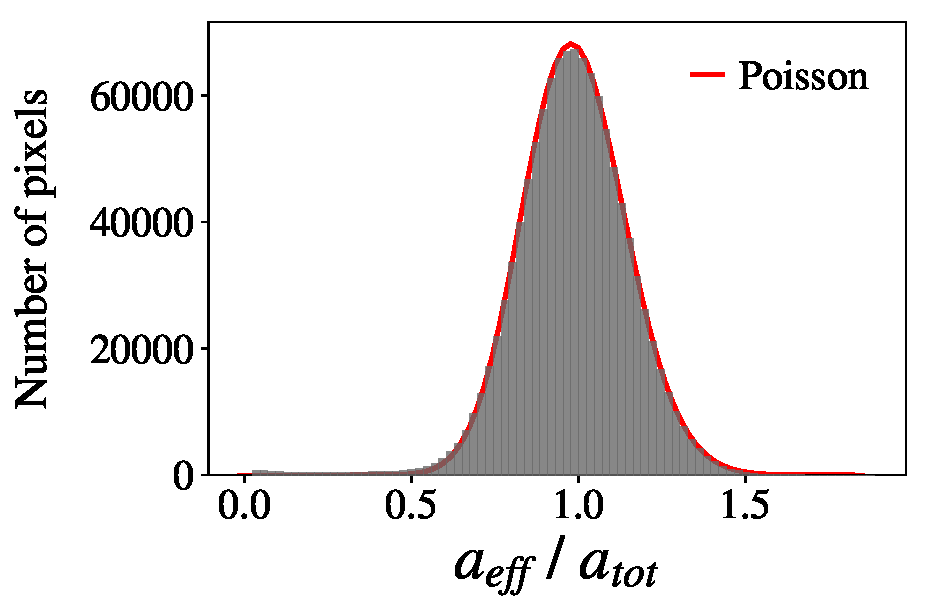
\includegraphics[width=0.85\columnwidth, trim={0.1cm 0 0 0},clip]{figures/poisson.pdf}  
    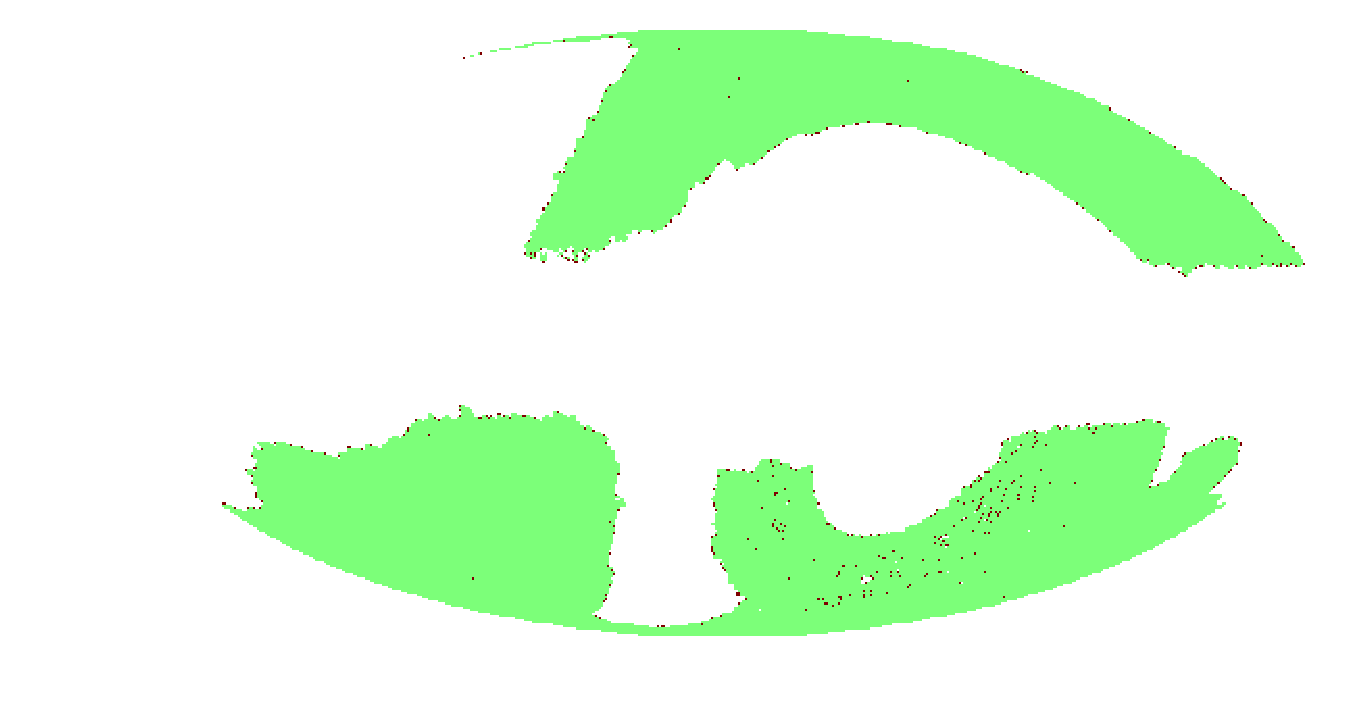
\includegraphics[width=\columnwidth]{figures/boundary.pdf}
    \caption{Upper: Histogram of the effective areas of pixels created with \texttt{HEALPix} resolution $N_{\rm SIDE} = 512$, showing a slight deviation from a Poisson distribution at the low end due to pixels straddling the footprint boundary or holes from the galaxy mask. Lower: Pixels selected as $a_{\rm eff}/a_{\rm tot} < 0.5$ lie predominately on the edges of the footprint.}
    \label{fig:desi_mask}
\end{figure}

The galaxy density map and mask are then upgraded to $N_{\rm SIDE} = 2048$ to match the resolution of the Planck CMB lensing map and mask, and converted from equatorial to galactic coordinates. To improve the stability of the matrix inversion, the Planck mask is apodized using a $1^{\circ}$ FWHM Gaussian\footnote{\citealt{Krolewski19} determined this to be the optimal smoothing scale for the Planck mask by testing on Gaussian simulations.}. The resulting masked galaxy density and CMB lensing convergence maps are shown in Figure~\ref{fig:pixel_maps}.

\begin{figure}
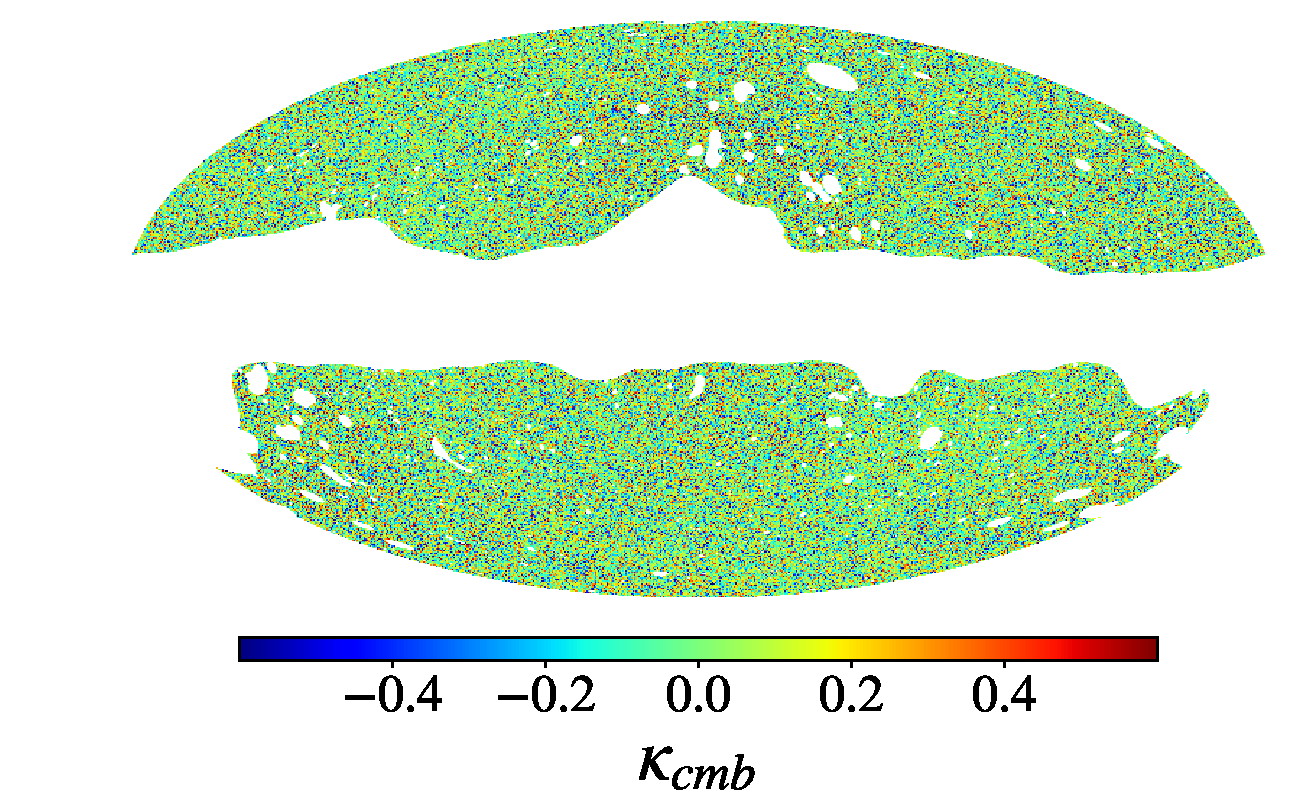
\includegraphics[width=\linewidth]{figures/cmb_map.pdf} 
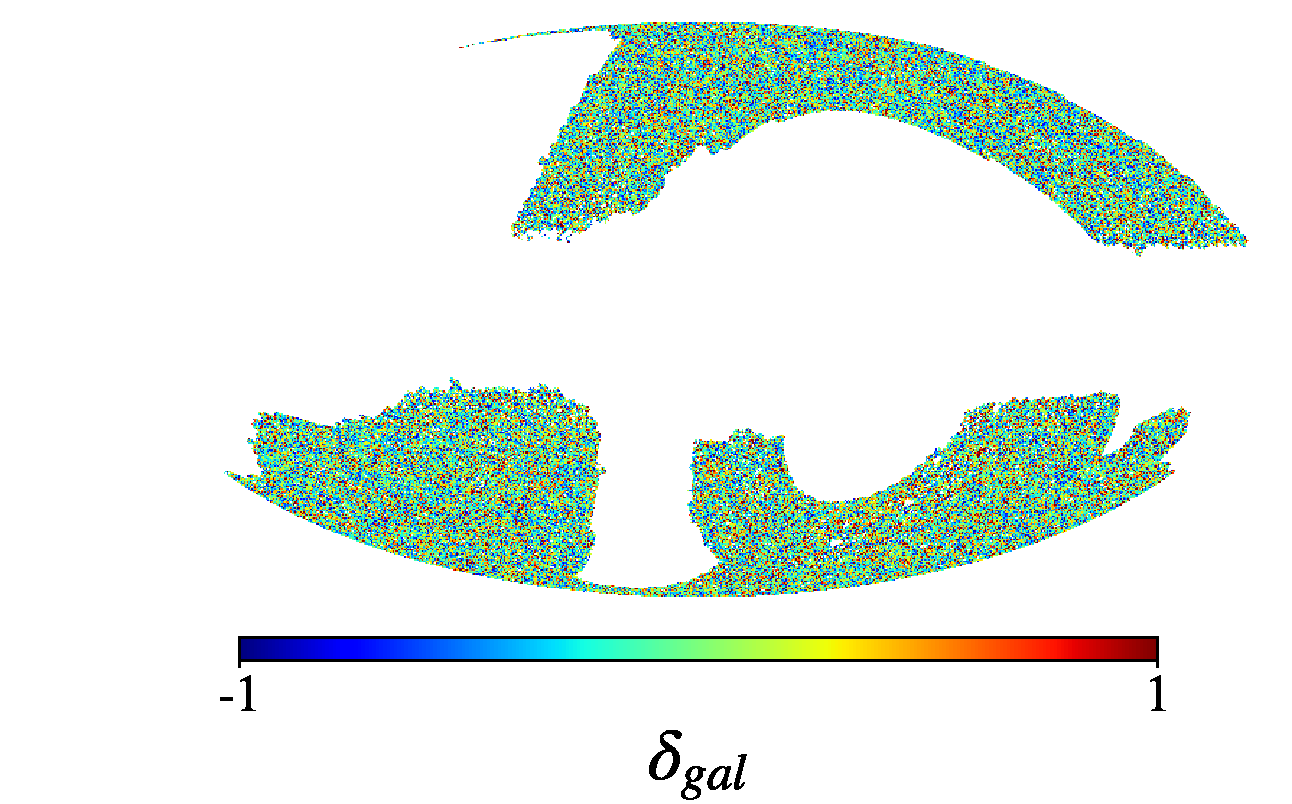
\includegraphics[width=\linewidth]{figures/gal_map.pdf}
\caption{Maps of Planck \texttt{BASE} CMB lensing convergence (upper) and DESI LRG galaxy overdensity (lower) in galactic coordinates, using \texttt{HEALPix} scheme with resolution $N_{\rm SIDE} = 2048$, Mollweide projection, and the astronomy convention (east towards left). Both maps are multiplied by their corresponding masks. The CMB lensing convergence is additionally smoothed on a scale of 10 arcmin for visual clarity.}
\label{fig:pixel_maps}
\end{figure}

% E.g. see Fig 1 of https://arxiv.org/pdf/1410.4502.pdf
%\textcolor{red}{Plots of $C_{\rm gg}, C_{g\kappa}, C_{\kappa\kappa}$ With error bars. With magnification bias errors too. With theory fits on top.}

%\subsection{Testing General Relativity?}

%In the Newtonian gauge, the line element corresponding to scalar perturbations of the Friedmann-Lema\^itre-Robertson-Walker spacetime metric may be written as
%\begin{equation}
%ds^2 = - \ (1 + 2 \Psi) \ dt^2 + a(t)^2 (1 - 2\Phi) \ d\Vec{x}^2
%\end{equation}
%where $a(t)$ is the scale factor, $d\Vec{x}^2 = d\chi^2 + D_A(\chi)^2d\Omega^2$ is the spatial element broken into line-of-sight and angular components, and $\Psi$ and $\Phi$ are the  potentials describing, respectively, the time-time and space-space deviations.
%\EK{TBC}

%\subsection{$\sigma_8(z)$ and $f_{NL}$?}
%\EK{TBC}


%If the dominant components of the stress-energy tensor have negligible anisotropic stress, then the Einstein equation of GR predicts that $\Psi = \Phi$, i.e., the same gravitational potential governs the time-time and space-space components of the metric. Anisotropic stress should be negligible in the matter-dominated era, and most proposed forms of dark energy (e.g., scalar fields) also have negligible anisotropic stress. Therefore, one generic form of modified gravity test is to check for the GR-predicted consistency between $\Psi$ and $\Phi$. For example, if the Ricci curvature scalar $R$ in the GR spacetime action is replaced by a function $f(R)$, then $\Psi$ and $\Phi$ are generically unequal. 

%%%

%By cross-correlating CMB lensing with other tracers such as galaxies, we can probe the evolution of the linear growth function, which is sensitive to deviations from GR.

%We can also test that the space-space and time-time components of the metric are equal as Einstein's theory predicts [the famous ``factor of 2'' in Einstein's bending of light formula].



%Let the spectroscopic sample have a known redshift distribution $dN_s/dz$.To calculate this, we bin the reference sample into narrow redshift bins $\delta z_i$. Then, for each $\delta z_i$, we estimate $w_{ur}(\theta,z_i)$ by pair counting with the Davis-Peebles estimator Equation~\ref{eqn:DPestimator}. In practice, we actually integrate over an annulus around each reference object, from $\theta_{\text{min}}$ to $\theta_{\text{max}}$, because the sensitivity of the estimator is improved by encoding information from many clustering scales \citep{Menard13}. In order to maximize the SNR, we weight each point by $\theta^{-1}$, which gives equal amounts of clustering information per logarithmic scale ($d\theta/\theta = d\log{\theta}$). 
%
%\begin{equation}
%\bar{w}_{ps}(z) \equiv  %\int_{\theta_{\text{min}}}^{\theta_{\text{max}}}{d\theta \ \frac{w_{ps}(\theta, z)}{\theta}} \propto b(z) \frac{dN_p}{dz}
%\end{equation}
%
% (estimated to be $\sim$0.03 arcseconds for DECaLS)
%To avoid excess signal from cross-correlations between duplicate objects that appear in both catalogs, it is necessary to impose a minimum radius, $\theta_{\text{min}}$ which is at least as large as the astrometric uncertainties in the survey. Furthermore, as we go to smaller scales $<$ 1 Mpc, clustering becomes increasingly nonlinear and bias becomes increasingly scale-dependent, so the assumptions underpinning the estimator break down, potentially affecting the accuracy of the result. Finally, we note that as the scale falls below the mean separation of spectroscopic objects, cross-correlations between redshift bins become more significant. Meanwhile, at larger scales, the advantage of a linear bias\footnote{The bias measured by these angular cross-correlations is dominated by scales of hundreds of kpc to a few Mpc, and thus should be distinguished from the large-scale ($>$10 Mpc) bias, which may evolve differently.} must be balanced against the cost of degraded signal-to-noise since the clustering signal decreases with radius and the noise due to systematics increases as more background sources are included in the counts. Thus, for samples which have little to no bias evolution, small scales are ideal for recovering $dN/dz$; for samples with some bias evolution, intermediate scales are recommended; and for samples with extensive bias evolution, restricting to large scales may be the best strategy.